% ---------------------------------------------------------------------------
% AXI MCDMA (PG288): vista simple. Un unico motor y un unico par de interfaces
% AXI-Stream dan servicio a los N perifericos; el campo TDEST del stream marca
% a que canal (y a que buffer de la DDR) pertenece cada paquete.
% Fuente del PDF que incluye la memoria (capitulo 2).
%
% Compilar:  pdflatex diagrama_mcdma.tex
% ---------------------------------------------------------------------------
\documentclass[border=8pt]{standalone}
\usepackage[utf8]{inputenc}
\usepackage[T1]{fontenc}
\usepackage{lmodern}
\usepackage{tikz}
\usetikzlibrary{arrows.meta, calc}

\definecolor{cIP}{HTML}{EDA100}       % ambar: IP de terceros (el MCDMA)
\definecolor{cExt}{HTML}{1BAF7A}      % aguamarina: resto del sistema
\definecolor{cRef}{HTML}{8A8A85}      % gris: lineas y rotulos

\tikzset{
    box/.style   ={draw, line width=0.9pt, rounded corners=2pt, align=center,
                   font=\sffamily\small, inner sep=4pt},
    ip/.style    ={box, draw=cIP!85!black, fill=cIP!12},
    ext/.style   ={box, draw=cExt!80!black, fill=cExt!10},
    buf/.style   ={draw=cExt!55!black, line width=0.5pt, rounded corners=1.5pt,
                   fill=cExt!4, minimum width=2.0cm, minimum height=0.55cm,
                   font=\sffamily\scriptsize},
    data/.style  ={{Stealth[length=6pt]}-{Stealth[length=6pt]},
                   line width=1.7pt, cRef!60!black},
    sax/.style   ={{Stealth[length=5pt]}-{Stealth[length=5pt]},
                   line width=1.1pt, cRef!58!black},
    ctrl/.style  ={-{Stealth[length=5pt]}, line width=0.8pt, cRef!80!black},
    irq/.style   ={-{Stealth[length=5pt]}, line width=0.8pt, cIP!70!black},
    rot/.style   ={font=\sffamily\scriptsize, text=cRef!45!black, inner sep=2pt},
}
\newcommand{\sub}[1]{{\scriptsize\textcolor{cRef!30!black}{#1}}}

\begin{document}
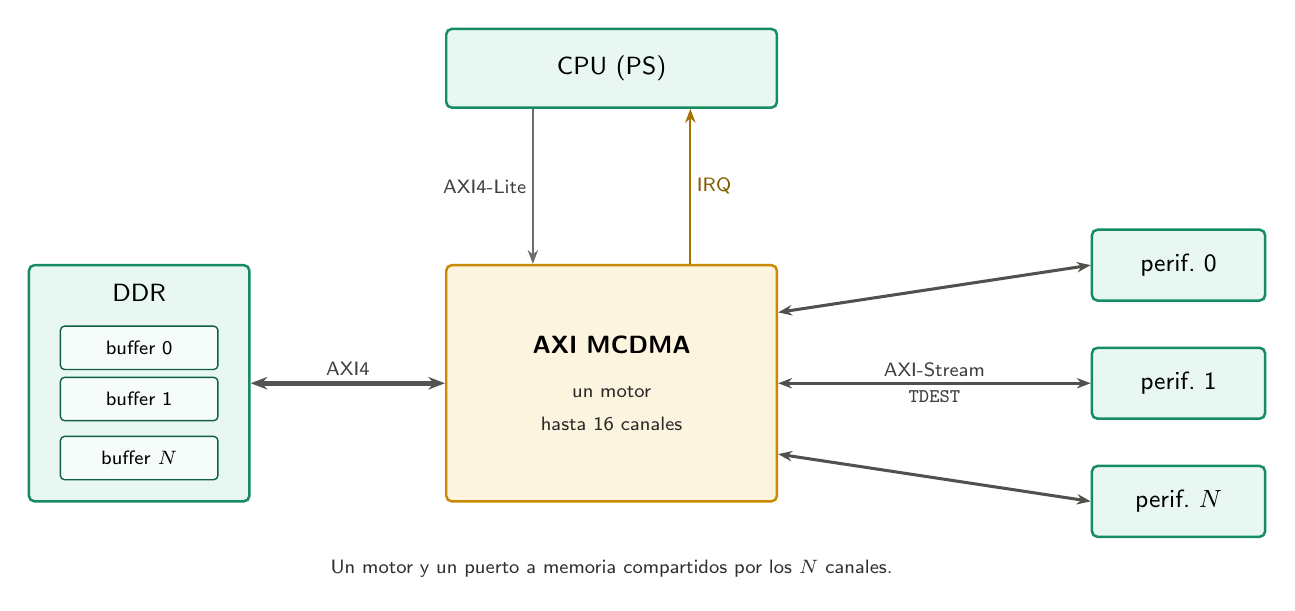
\begin{tikzpicture}[x=1cm, y=1cm]

% ===================== DDR con un buffer por canal =====================
\node[ext, minimum width=2.8cm, minimum height=3.0cm] (ddr) at (0,0) {};
\node[font=\sffamily\small] at (0,1.15) {DDR};
\node[buf] at (0,0.45)  {buffer 0};
\node[buf] at (0,-0.20) {buffer 1};
\node[buf] at (0,-0.95) {buffer $N$};

% ===================== MCDMA: un solo motor =====================
\node[ip, minimum width=4.2cm, minimum height=3.0cm] (mc) at (6,0)
     {\textbf{AXI MCDMA}\\[5pt]\sub{un motor}\\[1pt]\sub{hasta 16 canales}};

% ===================== CPU, aparte =====================
\node[ext, minimum width=4.2cm, minimum height=1.0cm] (cpu) at (6,4.0) {CPU (PS)};

% ===================== Perifericos: un AXI-Stream cada uno =====================
\node[ext, minimum width=2.2cm, minimum height=0.9cm] (p0) at (13.2, 1.5) {perif.\ 0};
\node[ext, minimum width=2.2cm, minimum height=0.9cm] (p1) at (13.2, 0.0) {perif.\ 1};
\node[ext, minimum width=2.2cm, minimum height=0.9cm] (pN) at (13.2,-1.5) {perif.\ $N$};
\draw[sax] (p0.west) -- ($(mc.east)+(0,0.9)$);
\draw[sax] (p1.west) -- (mc.east)
      node[midway, above, rot] {AXI-Stream}
      node[midway, below, rot] {\ttfamily TDEST};
\draw[sax] (pN.west) -- ($(mc.east)+(0,-0.9)$);

% ===================== Caminos de datos =====================
\draw[data] (ddr.east) -- (mc.west) node[midway, above, rot] {AXI4};

% ===================== Configuracion e interrupcion =====================
\draw[ctrl] ($(cpu.south)+(-1.0,0)$) -- ($(mc.north)+(-1.0,0)$)
      node[midway, left, rot] {AXI4-Lite};
\draw[irq]  ($(mc.north)+(1.0,0)$) -- ($(cpu.south)+(1.0,0)$)
      node[midway, right, rot, text=cIP!55!black] {IRQ};

% ===================== Idea clave =====================
\node[rot, text=cRef!35!black] at (6,-2.35)
     {Un motor y un puerto a memoria compartidos por los $N$ canales.};

\end{tikzpicture}
\end{document}
